%%%%%%%%%%%%%
\begin{singlespace}
\section{Aplication to Synthetic Data}

\noindent{In order to test the efficiency of the proposed inversion method, we applied it to two sets of synthetic data contaminated by high and/or low frequency noise. }

\noindent{The first synthetic test is performed by generating a simple set of four spheres with similar magnetization intensity and radius, but completely different magnetization directions. Generating a data set contaminated by high frequency noise. In this simulation, the magnetization directions and magnetic moment intensity are directly compared with the initial input parameters. This first simplified test is basically done to investigate the efficiency of the inversions used for Euler positioning and magnetization parameters, thus being a validation of the methodology.}

\noindent{The second data set is data generated by a more complex model containing one hundred spheres with different radius and magnetization intensity, but magnetized in a similar direction within one standard deviation. This data set is corrupted by both low and high frequency noise. In this second application there is also validation using the comparison of the model data with the retrieved data. The complexity of this synthetic data seeks to more faithfully simulate the applicability of the proposed method to real SMM data.}


%%%
\subsection{Simple Simulation: Validating the Methodology}

\noindent{We applied the proposed method in a numerical simulation of a geological thin-section of dimensions 1000 μm x 1000 μm in a regular grid (1000 x 1000) for estimating the magnetization directions of four spherical sources uniformly magnetized (but with different directions), according to \cref{tab:SimpleSyntheic}. Totaling an observation number N = $10^6$ obtained at a sensor-sample distance of 5 μm and a grid spacing of 1 μm. Subsequently, the data vector was contaminated with a pseudo-random noise of normal Gaussian distribution with a zero mean and 15 nT standard deviation, as shown in \cref{fig:SimpleSynthetic}a.}

\bigskip

\floatsetup[table]{capposition=top} % to put the caption on the top of the table
% If you use beamer only pass "xcolor=table" option, i.e. \documentclass[xcolor=table]{beamer}

\begin{table}[htbp]
\caption{Each source positioning and magnetization parameters modelled and recovered using least square estimator, respectively.}
\label{tab:SimpleSyntheic}
\resizebox{1.0\textwidth}{!}{
\begin{tabular}{ccccccc}
\hline   
\rowcolor[HTML]{FFFFFF} 
\cellcolor[HTML]{FFFFFF}                         & \multicolumn{3}{c}{\cellcolor[HTML]{FFFFFF}Center coordinates} & \multicolumn{3}{c}{\cellcolor[HTML]{FFFFFF}Magnetization}    \\
\rowcolor[HTML]{FFFFFF} 
\multirow{-2}{*}{\cellcolor[HTML]{FFFFFF}Sphere} & Xc ($\mu   m$)     & Yc ($\mu   m$)     & Zc ($\mu   m$)    & m ($A \cdot m^2$)       & D (\textdegree)          & I (\textdegree)           \\  \hline 
\multirow{2}{*}{1}                               & 250.00                 & 250.00                 & 5.30                & \multicolumn{1}{l}{8.70e-15}  & \multicolumn{1}{l}{-140.00}   & \multicolumn{1}{l}{-30.00}    \\ 
                                                 & 250.03                 & 249.94                 & 5.37                & 8.80e-15  $\pm$  1.39e-17           & -140.22  $\pm$  0.11            & -30.04    $\pm$  0.08           \\  \hline 
\multirow{2}{*}{2}                               & 500.00                 & 500.00                 & 7.75                & \multicolumn{1}{l}{7.63e-15}  & \multicolumn{1}{l}{-70.00}   & \multicolumn{1}{l}{-50.00}    \\ 
                                                 & 499.96                 & 500.00                 & 7.76                & 7.65e-15  $\pm$  1.89e-17           & -69.42  $\pm$  0.26            & -49.85    $\pm$  0.15           \\  \hline 
\multirow{2}{*}{3}                               & 750.00                 & 750.00                 & 8.50                & \multicolumn{1}{l}{6.21e-15}  & \multicolumn{1}{l}{10.00}   & \multicolumn{1}{l}{62.00}    \\
                                                 & 749.98                 & 749.97                 & 8.56                & 6.29e-15  $\pm$  1.98e-17           & 9.06  $\pm$  0.50            & 62.34    $\pm$  0.22           \\  \hline 
\multirow{2}{*}{4}                               & 200.00                 & 800.00                 & 10.00                & \multicolumn{1}{l}{4.97e-15}  & \multicolumn{1}{l}{125.00}   & \multicolumn{1}{l}{22.00}    \\
                                                 & 200.10                 & 800.12                 & 9.99                & 4.92e-15  $\pm$  3.00e-17           & 124.63  $\pm$  0.39            & 21.76    $\pm$  0.27           \\  \hline
\end{tabular}
}
\end{table}




\bigskip

\noindent{The first step is to apply the upward continuaton filter, which transforms the potencial field measured on a surface into one measured at a higher surface level \citep{Blakely1996}, therefore smoothing out high frequency noise. This first step is always needed in high frequency noisy data, since the Euler equation requires the first derivatives of potencial field. If this step is negleted or badly elaborated, the high frequency noise propagation during the application of the derivative filters will cause future errors in the next methodological stage.} 

\noindent{The next step is to calculate the magnetic total gradient (or horizontal gradient) filter in order to highlight the anomaly signal of each source within its own boundaries, then we apply the blob detection algorithm \citep{VanderWalt2014} to obtain a robust positioning of each source data window (\cref{fig:SimpleSynthetic}b).}

\begin{figure}[htbp]
\centering
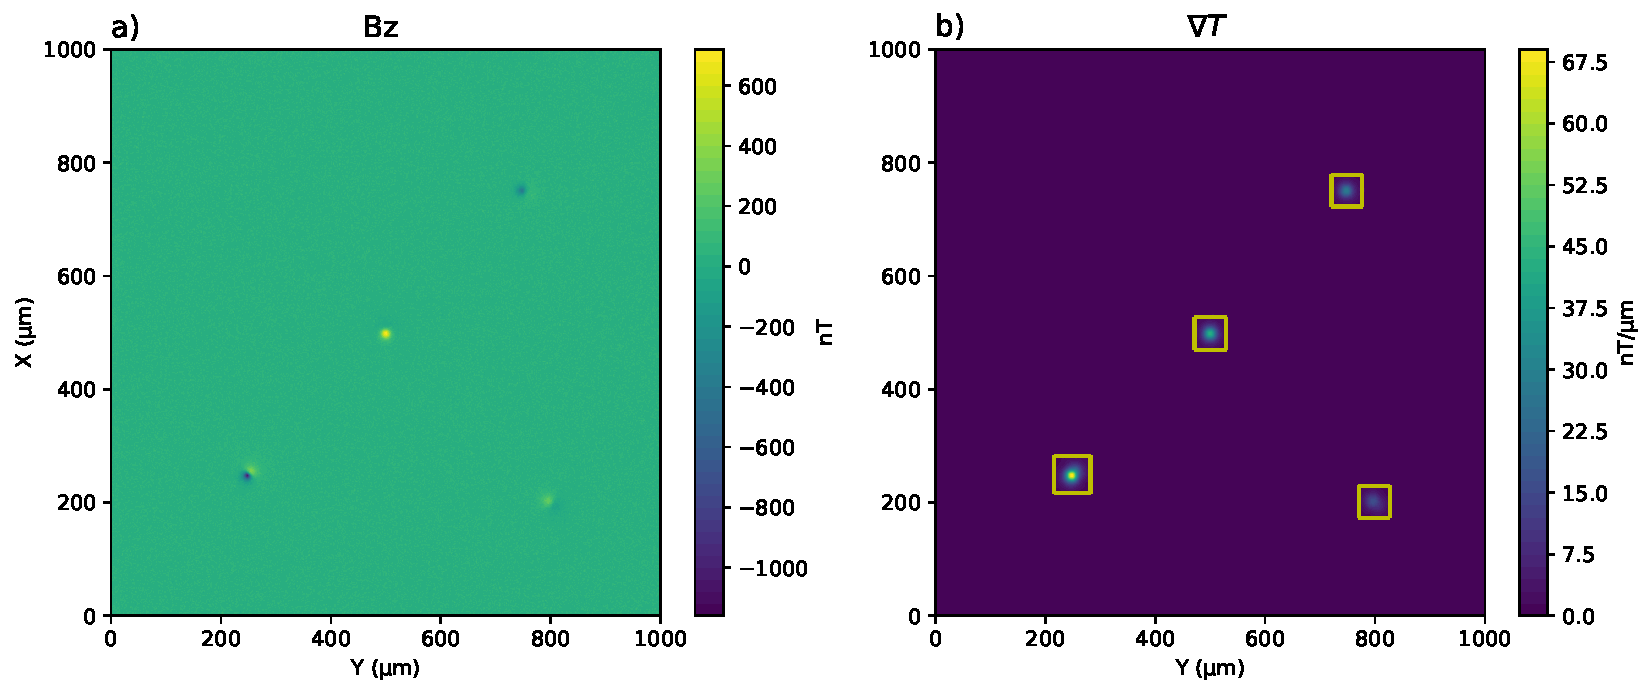
\includegraphics[width=1.0\textwidth]{SimpleSynthetic.png}
\caption{a) Synthetic data contaminated with psedo-random normal noise. b) Individual sources window position (yellow squares) obtained with the blob detection algorithm applied on the total gradient map.}
\label{fig:SimpleSynthetic}
\end{figure}

\bigskip

\noindent{After isolante the potencial field data and first derivatives for each source, we can solve the 3D Euler deconvolution \cref{eq:euler2} proposed by  \cite{Reid1990}, one for each subarea selected (window data), by assuming the structural index of a sphere/punctual source ($n = 3$). Thus, obtaining a sturdy result for the central positioning (Xc, Yc, Zc) of each source causing the magnetic potential anomaly in the observed data set, as shown in \cref{tab:SimpleSyntheic}.}

\noindent{The last step consists of using the central positions of each source, obtained with Euler's method, as an input parameter for inverting the original noisy data (\cref{fig:SimpleSynthetic}a) to find the least squares (or robust) approximation solution for the vector of cartesian magnetic moments ($\bar{m}$). With this, the magnetization directions (D and I) and the intensity of the magnetic moment can be estimated using equations (\cref{eq:sphere16,eq:sphere17,eq:sphere17_m}), as well as the uncertainty propagation of this inversion, using equations (\cref{eq:sphere21,eq:sphere22,eq:sphere22_m}) and considering $\sigma$ = 25nT. The results obtained with the least squares estimator can also be seen in \cref{tab:SimpleSyntheic}.}


\noindent{It is important to emphasize that \cite{OliveiraJr.2015} proved that the magnetization directions (D and I) recovered by the least squares estimator is sensitive to variations in the horizontal coordinates (x and y) of the magnetic sources central positions. While, the same being practically insensitive to variations in depths. Thus, the same authors consider Euler deconvolution method as an adequate technique to estimate the central positions that will be used as a priori information for inversion. This occurs mainly because, when well performed, the recovery of the horizontal coordinates of sources central position is considerably accurate, while the vertical coordinate can undergo greater variation \citep{Silva2003, Melo2013}, even so the inversion will still provide extremely satisfactory results. The high sensitivity of Euler deconvolution to high frequency noise can also be easily overcome with the proper application of the upward continuation filter.}




\subsection{Complex Simulation: Testing Applicability}

\begin{figure}[hbpt]
\centering
\includegraphics[width=1.0\textwidth]{ComplexSynthetic.png}
\caption{a) Complex synthetic data contaminated with  both high and low frequencies noise. b) Individual sources window position (yellow squares) obtained with the blob detection algorithm applied on the total gradient map.}
\label{fig:ComplexSynthetic}
\end{figure}


\begin{figure}[hbpt]
\centering
\includegraphics[width=1.0\textwidth]{ComplexComparison.png}
\caption{blablabla.}
\label{fig:ComplexSynthetic2}
\end{figure}

\begin{figure}[hbpt]
\centering
\includegraphics[width=1.0\textwidth]{ComplexStereo.png}
\caption{blablabla.}
\label{fig:ComplexSynthetic3}
\end{figure}

\end{singlespace}